%%%%%%%%%%%%%%%%%%%%%%%%%%%%
% Two Sword Lengths Apart: Supplementary Material
% 15 February 2014
%%%%%%%%%%%%%%%%%%%%%%%%%%%%

% !Rnw weave = knitr

\documentclass[a4paper]{article}\usepackage[]{graphicx}\usepackage[]{color}
%% maxwidth is the original width if it is less than linewidth
%% otherwise use linewidth (to make sure the graphics do not exceed the margin)
\makeatletter
\def\maxwidth{ %
  \ifdim\Gin@nat@width>\linewidth
    \linewidth
  \else
    \Gin@nat@width
  \fi
}
\makeatother

\definecolor{fgcolor}{rgb}{0.345, 0.345, 0.345}
\newcommand{\hlnum}[1]{\textcolor[rgb]{0.686,0.059,0.569}{#1}}%
\newcommand{\hlstr}[1]{\textcolor[rgb]{0.192,0.494,0.8}{#1}}%
\newcommand{\hlcom}[1]{\textcolor[rgb]{0.678,0.584,0.686}{\textit{#1}}}%
\newcommand{\hlopt}[1]{\textcolor[rgb]{0,0,0}{#1}}%
\newcommand{\hlstd}[1]{\textcolor[rgb]{0.345,0.345,0.345}{#1}}%
\newcommand{\hlkwa}[1]{\textcolor[rgb]{0.161,0.373,0.58}{\textbf{#1}}}%
\newcommand{\hlkwb}[1]{\textcolor[rgb]{0.69,0.353,0.396}{#1}}%
\newcommand{\hlkwc}[1]{\textcolor[rgb]{0.333,0.667,0.333}{#1}}%
\newcommand{\hlkwd}[1]{\textcolor[rgb]{0.737,0.353,0.396}{\textbf{#1}}}%

\usepackage{framed}
\makeatletter
\newenvironment{kframe}{%
 \def\at@end@of@kframe{}%
 \ifinner\ifhmode%
  \def\at@end@of@kframe{\end{minipage}}%
  \begin{minipage}{\columnwidth}%
 \fi\fi%
 \def\FrameCommand##1{\hskip\@totalleftmargin \hskip-\fboxsep
 \colorbox{shadecolor}{##1}\hskip-\fboxsep
     % There is no \\@totalrightmargin, so:
     \hskip-\linewidth \hskip-\@totalleftmargin \hskip\columnwidth}%
 \MakeFramed {\advance\hsize-\width
   \@totalleftmargin\z@ \linewidth\hsize
   \@setminipage}}%
 {\par\unskip\endMakeFramed%
 \at@end@of@kframe}
\makeatother

\definecolor{shadecolor}{rgb}{.97, .97, .97}
\definecolor{messagecolor}{rgb}{0, 0, 0}
\definecolor{warningcolor}{rgb}{1, 0, 1}
\definecolor{errorcolor}{rgb}{1, 0, 0}
\newenvironment{knitrout}{}{} % an empty environment to be redefined in TeX

\usepackage{alltt}
\usepackage{fullpage}
\usepackage{lscape}
\usepackage[authoryear,comma]{natbib}
\usepackage{setspace}
    \doublespacing
\usepackage{hyperref}
\hypersetup{
    colorlinks,
    citecolor=black,
    filecolor=black,
    linkcolor=cyan,
    urlcolor=cyan
}
\usepackage{booktabs}
\usepackage{dcolumn}
\usepackage{url}
\usepackage{tikz}
\usepackage{todonotes}
\usepackage{verbatim}
\usepackage{endnotes}
\usepackage{graphicx}

\usepackage{footmisc}
\setlength{\footnotesep}{\baselineskip}
\renewcommand{\footnotelayout}{\doublespacing\normalsize}

\setlength{\belowcaptionskip}{0.5cm}

%%%%%%% Title Page %%%%%%%%%%%%%%%%%%%%%%%%%%%%%%%%%%%%%%%%%%%%
\title{Supplementary Material: Two Sword Lengths Apart: Credible Commitment Problems and Physical Violence in Multi-party Elected National Legislatures}
\IfFileExists{upquote.sty}{\usepackage{upquote}}{}
                
\begin{document}

\maketitle



%%%%%%%%%%%%%%%% Run Analyses %%%%%%%%%%%%%%%%%%%%%%%%




\subsection*{Details on Prior Correction of the Rare Logistic Regression Models}

For prior correction\footnote{\citep[see][]{KingRareEventsPA2001}} in the models with the full sample of elected multi-party legislatures I used the observed proportion of all observations with legislative violence up to 2010: i.e. 2 percent of observations up until 2010 had violence ($\tau = \frac{77}{3830} = 0.02$). There were 69 observed incidences of violence and 2927 country-years from 1990 through 2009 in the sample, so: $\tau = \frac{69}{2927} = 0.024$.



%%%%%%%% Elected Legislatures Results Table
\begin{table}
\caption{Legislative Violence Rare Events Logistic Regression Results (Multi-Party Elected Legislature 1981-2009)}
\label{outputTable.dem}
\begin{center}
\scalebox{0.9}{

\begin{tabular}{l c c c c c c c c }
\hline
                        & B1 & B2 & B3 & B4 & B5 & B6 & B7 & B8 \\
\hline
(Intercept)             & $-2.85^{***}$ & $-1.23$       & $-3.45$       & $-1.46^{*}$  & $-2.36^{**}$ & $-1.83^{*}$  & $-1.80^{*}$   & $-1.77$      \\
                        & $(0.20)$      & $(0.77)$      & $(4.33)$      & $(0.65)$     & $(0.85)$     & $(0.84)$     & $(0.76)$      & $(1.00)$     \\
Low Disproportionality  & $-1.31^{***}$ & $-1.67^{***}$ & $-2.17^{***}$ & $-1.11^{**}$ & $-1.27^{*}$  & $-1.53^{**}$ & $-1.43^{***}$ & $-1.13^{**}$ \\
                        & $(0.34)$      & $(0.35)$      & $(0.62)$      & $(0.38)$     & $(0.53)$     & $(0.57)$     & $(0.37)$      & $(0.37)$     \\
Dem. Age                & $-0.02^{**}$  & $-0.02^{**}$  & $-0.02$       & $-0.02^{*}$  & $-0.03^{*}$  & $-0.03^{*}$  & $-0.02^{**}$  & $-0.02^{*}$  \\
                        & $(0.01)$      & $(0.01)$      & $(0.01)$      & $(0.01)$     & $(0.01)$     & $(0.01)$     & $(0.01)$      & $(0.01)$     \\
Majority Size           &               & $-0.03^{***}$ & $-0.02$       & $-0.02^{*}$  & $0.00$       & $-0.02$      & $-0.03^{*}$   & $-0.02^{*}$  \\
                        &               & $(0.01)$      & $(0.01)$      & $(0.01)$     & $(0.01)$     & $(0.01)$     & $(0.01)$      & $(0.01)$     \\
Leg. Immunity           &               & $-0.37$       &               &              &              &              &               &              \\
                        &               & $(0.33)$      &               &              &              &              &               &              \\
PR Electoral System     &               & $1.06^{*}$    &               &              &              &              &               &              \\
                        &               & $(0.51)$      &               &              &              &              &               &              \\
Single Party Gov.       &               & $-0.53$       &               &              &              &              &               &              \\
                        &               & $(0.31)$      &               &              &              &              &               &              \\
Self Expression         &               &               & $1.48$        &              &              &              &               &              \\
                        &               &               & $(3.44)$      &              &              &              &               &              \\
Ethnic Frac.            &               &               & $0.81$        &              &              &              &               &              \\
                        &               &               & $(1.09)$      &              &              &              &               &              \\
Perc. Women in Parl.    &               &               &               & $-0.02$      &              &              &               &              \\
                        &               &               &               & $(0.02)$     &              &              &               &              \\
Murder Rate             &               &               &               &              & $0.01$       &              &               &              \\
                        &               &               &               &              & $(0.02)$     &              &               &              \\
Federal                 &               &               &               &              &              & $0.74$       & $0.79^{*}$    &              \\
                        &               &               &               &              &              & $(0.60)$     & $(0.39)$      &              \\
Gov. Frac.              &               &               &               &              &              & $0.79$       &               &              \\
                        &               &               &               &              &              & $(0.82)$     &               &              \\
No. of Parties by Seats &               &               &               &              &              &              & $0.12$        &              \\
                        &               &               &               &              &              &              & $(0.07)$      &              \\
GINI                    &               &               &               &              &              &              &               & $0.01$       \\
                        &               &               &               &              &              &              &               & $(0.02)$     \\
GDP per Capita          &               &               &               &              &              &              &               & $0.00$       \\
                        &               &               &               &              &              &              &               & $(0.03)$     \\
\hline
AIC                     & 443.72        & 425.38        & 215.80        & 370.34       & 191.36       & 176.05       & 367.64        & 353.38       \\
BIC                     & 460.95        & 465.48        & 244.39        & 398.19       & 215.19       & 204.71       & 401.24        & 386.08       \\
Log Likelihood          & -218.86       & -205.69       & -101.90       & -180.17      & -90.68       & -82.02       & -177.82       & -170.69      \\
Deviance                & 437.72        & 411.38        & 203.80        & 360.34       & 181.36       & 164.05       & 355.64        & 341.38       \\
Num. obs.               & 2306          & 2274          & 866           & 2274         & 1960         & 931          & 2053          & 2005         \\
\hline
\multicolumn{9}{l}{\scriptsize{\textsuperscript{***}$p<0.001$, 
  \textsuperscript{**}$p<0.01$, 
  \textsuperscript{*}$p<0.05$}}
\end{tabular}


}
\end{center}
{\scriptsize{
    Standard errors are in parentheses. All models use robust (WEAVE) standard errors. \\
}}
\end{table}



%%%%%%%%%%%%%%%%%%%%%% Figures Start %%%%%%%%%%%%%%%%%%%%%%%%%%%%%%%%%%%%%%%%%%%%%


%%%%%%%% Variable source summary table
\begin{table}[!h]
    \begin{center}
    \caption{Variable Summary}
    \label{var_summary}
    \begin{tabular}{l m{7cm} m{3.5cm}}

            \hline
            Variable & Description & Source \\
            \hline \hline
            Disprop & Gallagher Index of Electoral Disproportionality & \cite{Gallagher2012} \& \cite{Carey2011} \\
            ENPS & Effective number of parties by seats & \cite{Gallagher2012} \& \cite{Carey2011} \\
            ENPV & Effective number of parties by votes & \cite{Gallagher2012} \& \cite{Carey2011} \\
            Ethnic Fractionalization & Probability two randomly selected members of society are from the same ethnic group & \cite{Alesina2003} \\
            Federal & Whether a country has a federal system or not & \cite{Carey2011}, updated from 2003 by the author \\           
            GDP/Capita & GDP per capita in thousands of US dollars & \cite{WorldBank2011} \\
            Gov. Fractionalization & Probability that two members of the Government will be from different parties & \cite{DPI2001} \\
            Gini & Gini Coefficient of income inequality & \cite{UNU2008} \\
            Immunity & Whether a legislators are immune from arrest and/or criminal prosecution or not & \cite{Fish2009} \\
            LEIC & Legislative Indices of Electoral Competitiveness. Includes both the existence of a legislature and its level of electoral competitiveness. & \cite{DPI2001} \\
            Majority & Percentage of legislature controlled by governing parties & \cite{DPI2001} \\
            Murder Rate & Murders per 100,000 population & \cite{UNMurder2013} \\
            Polity & Polity IV Score & \cite{Marshall2009} \\
            PR & Whether a country uses a proportional representation electoral system or a plurality system & \cite{DPI2001} \\
            Self Expression & WVS self-expression indicator averaged across country-survey waves & \cite{WVS2009} \\
            System & Government system (parliamentary, presidential, or mixed & \cite{DPI2001} \\
            Tenshort & Tenure of the shortest serving veto player & \cite{DPI2001} \\
            Trust & Average of WVS responses where 1 $=$ most people can be trusted and 2 $=$ you can't be too careful & \cite{WVS2009} \\
            UDS & Posterior Mean Unified Democracy Score & \cite{Pemstein2010} \\
            Violence & Incidences of violence between legislators in the national parliamentary chamber & author \\
            Perc. Women in Parl. & Percentage of parliamentary seats held by women & \cite{WomParCrossNat} \& \cite{IPU2013} \\
            \hline

    \end{tabular}
    \end{center}
    \begin{singlespace}
        Please contact the author for detailed summary statistics. \\
        All of the data from \cite{DPI2001} was updated through 2010.
    \end{singlespace}
\end{table}  

%%%%%%%%%% Correlation matrix %%%%%%%%%% 
\begin{landscape}
\begin{figure}[t]
    \caption{Correlation Matrix for Variables Included in the Analysis (Multi-Party Elected Legislatures)}
    \label{corrmatrix}
    \begin{center}
    
    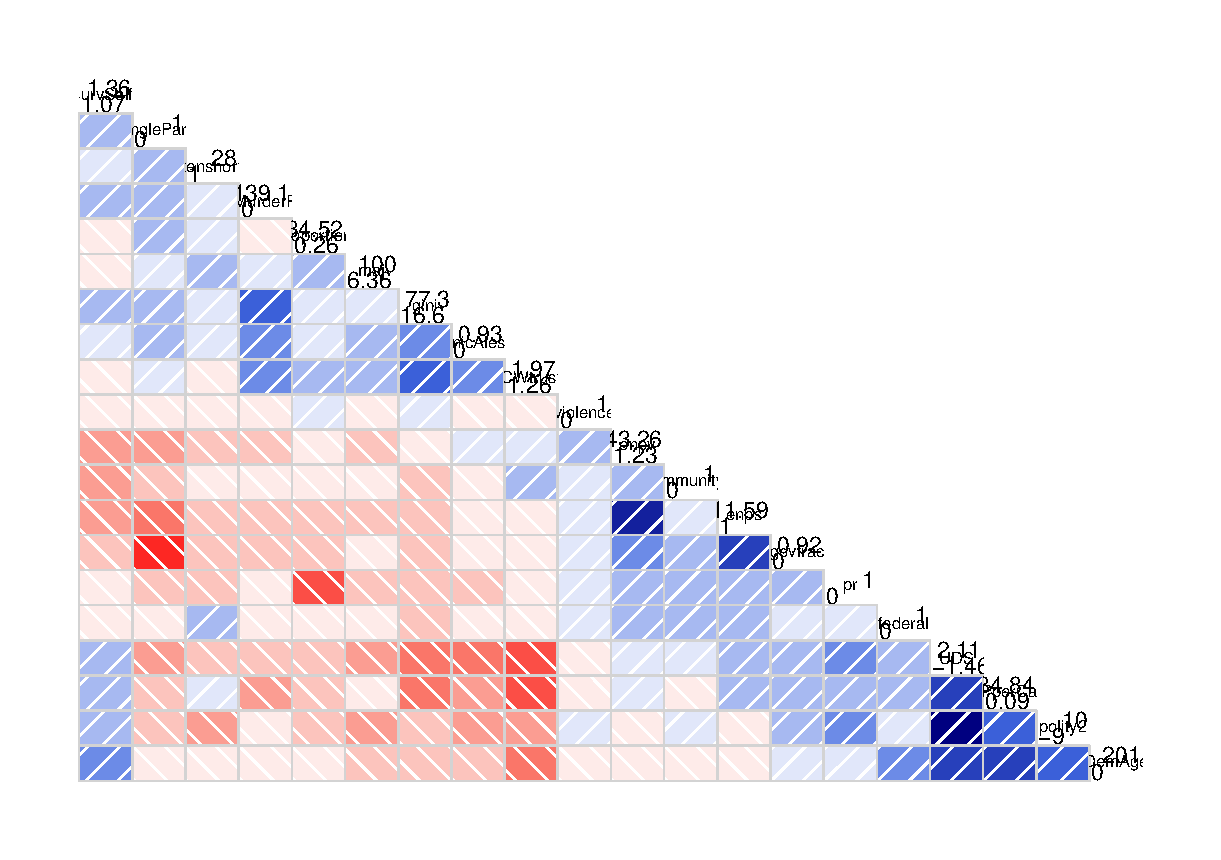
\includegraphics[width = \textwidth]{corrScatter.pdf}  
    %%% corScatter not created every compile to save time %%%
%<<corScatter>>=

%    library(corrgram)  

%    ### Create data set with variables for corrgram
%    vars.corrgram <- c("violence", "system", "DemAge", "maj", "MajCat", "govfrac", "singleParty", "pr", "tenshort", "UDS", "polity2", "ethnicAlesina", "CWtrust", "CWsurvSelfExpr", "disproportionality", "gini", "GDPperCapita", "enps", "enpv", "federal", "immunity", "UNMurderRate")

%    # Subset elected legislature data
%    dem.corrData <- dem[vars.corrgram]

%    # Create corrgram
%    dem.corrgram <- corrgram(dem.corrData, order = TRUE, upper.panel = NULL, diag.panel = panel.minmax)

%@

    \end{center}
    \begin{singlespace}
        {\scriptsize{Redder squares indicate stronger negative bi-variate correlations. \\
        Bluer squares indicate stronger positive bi-variate correlations. \\
        Numbers in the diagonal squares indicate the minimum and maximum observed values of the variables in the sample.
        }}
    \end{singlespace} 
\end{figure}
\end{landscape}

%%%%%%%%%%%%%%%%%%%%%% Figures End %%%%%%%%%%%%%%%%%%%%%%%%%%%%%%%%%%%%%%%%%%%%%

\bibliographystyle{apsr}
\bibliography{LegViolence}

\end{document}
